%%%%%%%%%%%%%%%%%%%%%%%%%%%%%%%%%%%%%%%%%
% Beamer Presentation
% LaTeX Template
% Version 1.0 (10/11/12)
%
% This template has been downloaded from:
% http://www.LaTeXTemplates.com
%
% License:
% CC BY-NC-SA 3.0 (http://creativecommons.org/licenses/by-nc-sa/3.0/)
%
%%%%%%%%%%%%%%%%%%%%%%%%%%%%%%%%%%%%%%%%%

%----------------------------------------------------------------------------------------
%	PACKAGES AND THEMES
%----------------------------------------------------------------------------------------

\documentclass{beamer}

\mode<presentation> {

% The Beamer class comes with a number of default slide themes
% which change the colors and layouts of slides. Below this is a list
% of all the themes, uncomment each in turn to see what they look like.

%\usetheme{default}
%\usetheme{AnnArbor}
%\usetheme{Antibes}
%\usetheme{Bergen}
%\usetheme{Berkeley}
%\usetheme{Berlin}
%\usetheme{Boadilla}
%\usetheme{CambridgeUS}
\usetheme{Copenhagen}
%\usetheme{Darmstadt}
%\usetheme{Dresden}
%\usetheme{Frankfurt}
%\usetheme{Goettingen}
%\usetheme{Hannover}
%\usetheme{Ilmenau}
%\usetheme{JuanLesPins}
%\usetheme{Luebeck}
%\usetheme{Madrid}
%\usetheme{Malmoe}
%\usetheme{Marburg}
%\usetheme{Montpellier}
%\usetheme{PaloAlto}
%\usetheme{Pittsburgh}
%\usetheme{Rochester}
%\usetheme{Singapore}
%\usetheme{Szeged}
%\usetheme{Warsaw}

% As well as themes, the Beamer class has a number of color themes
% for any slide theme. Uncomment each of these in turn to see how it
% changes the colors of your current slide theme.

%\usecolortheme{albatross}
%\usecolortheme{beaver}
%\usecolortheme{beetle}
%\usecolortheme{crane}
%\usecolortheme{dolphin}
%\usecolortheme{dove}
%\usecolortheme{fly}
%\usecolortheme{lily}
%\usecolortheme{orchid}
%\usecolortheme{rose}
%\usecolortheme{seagull}
%\usecolortheme{seahorse}
%\usecolortheme{whale}
%\usecolortheme{wolverine}

%\setbeamertemplate{footline} % To remove the footer line in all slides uncomment this line
%\setbeamertemplate{footline}[page number] % To replace the footer
%line in all slides with a simple slide count uncomment this line

%\setbeamertemplate{navigation symbols}{} % To remove the navigation
%symbols from the bottom of all slides uncomment this line
}

\usepackage{graphicx} % Allows including images
\usepackage{booktabs} % Allows the use of \toprule, \midrule and \bottomrule
                      % in tables

\DeclareGraphicsExtensions{.pdf,.png,.jpg}
\usepackage{amssymb,amsmath,amsthm,amsfonts}
\usepackage{mathrsfs}
\usepackage{dsfont}
\usepackage{enumerate}

%\newtheorem{mdef}{Definition}
%\newtheorem{theorem}{Theorem}
\newcommand{\eqsplit}[2]{
  \begin{equation}\label{#2}
    \begin{split}
      #1
    \end{split}
  \end{equation}}
\newcommand{\eqnsplit}[1]{
  \begin{eqnarray*}
    #1
  \end{eqnarray*}}
\newcommand{\tran}[1]{
  \tilde{#1}
}
\newcommand{\td}[2]{
  \frac{d #1}{d #2}
}
\newcommand{\pd}[2]{
  \frac{\partial #1}{\partial #2}
}
\newcommand{\ppd}[2]{
  \frac{\partial^2 #1}{\partial #2^2}
}
\newcommand{\pdd}[3]{
  \frac{\partial^2 #1}{\partial #2 \partial #3}
}
\newcommand{\otd}[1]{
  \frac{d}{d #1}
}
\newcommand{\opd}[1]{
  \frac{\partial}{\partial #1}
}
\newcommand{\oppd}[1]{
  \frac{\partial^2}{\partial #1^2}
}
\newcommand{\opdd}[2]{
  \frac{\partial^2}{\partial #1 \partial #2}
}
\newcommand{\ket}[1]{
  |#1\rangle
}
\newcommand{\bra}[1]{
  \langle#1|
}
\newcommand{\inn}[1]{
  \langle#1\rangle
}
\newcommand{\mean}[1]{
  \langle#1\rangle
}
\newcommand{\tr}{
  \text{tr}\,
}
\newcommand{\re}{
  \text{Re}\,
}
\newcommand\im{
  \text{Im}\,
}
\newcommand{\var}{
  \text{var}
}
\newcommand{\arcsinh}{
  \sinh^{-1}
}
\newcommand{\arccosh}{
  \cosh^{-1}
}
\newcommand{\erfc}{
  \text{erfc}
}
\newcommand{\E}{
  \mathbb{E}
}
\renewcommand{\P}{
  \mathbb{P}
}
\newcommand{\I}[1]{
  \mathbf{1}_{\{#1\}}
}
\newcommand{\1}[1]{
  \mathds{1}_{\{#1\}}
}
\newcommand{\diag}{
  \text{diag\,}
}
\newcommand{\M}{
  {\text{max}}
}
\newcommand{\m}{
  {\text{min}}
}
\newcommand{\ph}{
  {\text{arg}\,}
}
\newcommand\erf{
  \text{erf}
}
\renewcommand\vec[1]{
  \mathbf{#1}
}
\newcommand\mtx[1]{
  \mathbf{#1}
}
\newcommand\ed{
  \,{\buildrel d \over =}\,
}




%----------------------------------------------------------------------------------------
%	TITLE PAGE
%----------------------------------------------------------------------------------------

\title{An Efficient Estimator of 1D MC Exceedance Probability for Perpurtuities} % The
                                % short title appears at the bottom of
                                % every slide, the full title is only
                                % on the title page

\author{Xie Xiaolei} % Your name
\institute[UCPH] % Your institution as it will appear on the bottom of every slide, may be shorthand to save space
{
Copenhagen University  \\ % Your institution for the title page
\medskip
\textit{hnq365@math.ku.dk} % Your email address
}
\date{\today} % Date, can be changed to a custom date

\begin{document}

\begin{frame}
\titlepage % Print the title page as the first slide
\end{frame}

% \begin{frame}
% \frametitle{Overview}
% \tableofcontents
% \end{frame}

%----------------------------------------------------------------------------------------
%	PRESENTATION SLIDES
%----------------------------------------------------------------------------------------
% \section{Simple dependence models}
%------------------------------------------------
\section{Introduction}
\begin{frame}
  We are interested in the {\it Stochastic Fixed Point Equations}:
  \[
  V \overset{d}{=} f_Y(V)
  \]
  \begin{enumerate}
  \item Forward sequence
    \[
    V_n = f_{Y_n} \circ f_{Y_{n-1}} \circ \cdots \circ f_{Y_1} (V_0)
    \]
    \item Backward sequence
      \[
      Z_n  = f_{Y_1} \circ f_{Y_{2}} \circ \cdots \circ f_{Y_n} (Z_0)
      \]
    \end{enumerate}
    where $Y_i$ are iid copies of $Y$ and are termed environment
    variables. The {\it GARCH(1, 1)} model is a typical forward sequence.
    \begin{eqnarray*}
      V_n &=& \sigma_n^2 \\
      Y_n &=& \eta_{n-1} \\
      F_Y(v) &=& (\beta_1 + \alpha_1 Y_n^2) v + \alpha_0
    \end{eqnarray*}
\end{frame}

\begin{frame}
  Letac's Model E:
  \[
  V_n = A_n (V_{n-1} \vee D_n) + B_n
  \]
  where $(\log A_n, B_n, D_n)$ are iid.
\end{frame}

\begin{frame}
Assume:
\begin{enumerate}
\item $A$ is positive, absolutely continuous and has a non-trivial continuous density in
  a neighborhood of $\mathbb R$.
\item Define $\Lambda(\alpha) := \log \E A^\alpha$, $\Lambda(\xi) = 0$ for some $\xi \in (0,
  \infty)$ and $\Lambda(\cdot)$ is differentiable at $\xi$.
\item $\P(A > 1, B > 0) > 0$ or $P(A > 1, B \geq 0, D > 0) > 0$.
\item $\E |B|^\xi < \infty$, $\E (A|D|)^\xi < \infty$
\end{enumerate}
Under these conditions Goldie proved that a solution to the
SFPE satisfies
\[
\P(V > u) = C(u) u^{-\xi}
\]
for some constant $\xi$. As $u \to \infty$, $C(u)$ tends to a constant
$C$.
% In multidimensions, Kesten's theorem states, for the stochastic
% recurrence equation $V \overset{d}{=} A V + B$,
% \[
% \lim_{u \to \infty} u^\alpha \P(\inn{\tilde {x},V} > u) =
% g_{\alpha}(\tilde x)
% \]
% where $A \in \mathbb R^{d \times d}$, $V \in \mathbb R^d$ and $\tilde x \in
% \mathbb S^{d-1}$.
\end{frame}

\begin{frame}
  \begin{figure}[htb!]
    \centering
    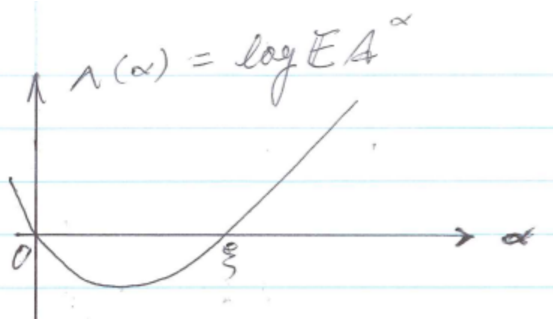
\includegraphics[scale=0.8]{pic2.pdf}
  \end{figure}
  The function $\Lambda(\alpha)$ is convex, passes through the origin
  and crosses the $\alpha$-axis at $\xi > 0$.
\end{frame}

\begin{frame}
  \begin{exampleblock}{Our Goal}
    Explicit numerical estimation of the probability $\P(V > u)$ for a
    forward sequence $V_n$.
  \end{exampleblock}
  \begin{exampleblock}{Why}
    Straight forward Mont-Carlo simulation is inefficient because
    $\P(V > u) \to 0$ as $u \to \infty$. A measure of the efficiency
    of estimator $\mathcal E_u$ is the relative error:
    \[
    \text{Relative Error} = {
      \var(\mathcal E_u)
      \over
      (\E \mathcal E_u)^2
    }
    \]
  \end{exampleblock}
  \begin{exampleblock}{The Idea}
    Change to the $\xi$ shifted measure of $\log A$, under which $V_n$ has
    been shown to be transient.
  \end{exampleblock}
\end{frame}

\begin{frame}
  \frametitle{An Efficient Estimator}
  \begin{block}{Theorem}
    \[
    \mathcal E_u = \pi(\mathcal C) \E_{\mathcal D} {N_u
      \over
      (A_{T_u} \cdots A_1)^\xi
    }\1{T_u < K}
    \]
    is an efficient estimator of $\P(V > u)$
  \end{block}
\end{frame}

\begin{frame}
  $\mathcal D$ denotes the dual measure:
  If $n < T_u$, i.e. the MC
  has not exceeded the level $u$, $A_{n+1}$ is sampled from the
  $\xi$-shifted distribution $\mu_\xi$; otherwise it is sampled from
  $\mu$. For a set $S \subseteq \text{supp}(A)$
  \begin{eqnarray*}
    \mu_\xi (S) &=& {
      \int_{S} a^\xi \mu(da)
      \over
      \int_{\text{supp}(A)} a^\xi \mu(da)
    } = {\E A^\xi \I{S}(A)
      \over
      \E A^\xi
    }
  \end{eqnarray*}
  Denote
  \begin{eqnarray*}
    \lambda(\alpha) &=& \E A^{\alpha} \\
    \lambda_\beta(\alpha) &=& \E_\beta A^{\alpha} = {
      \E A^{\alpha + \beta}
      \over
      \E A^{\beta}
    }
  \end{eqnarray*}  
\end{frame}

\begin{frame}
  \begin{figure}[htb!]
    \centering
    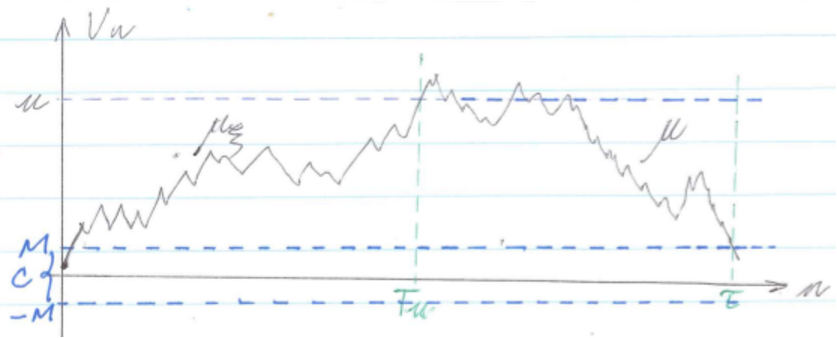
\includegraphics[scale=0.5]{pic1.pdf}
  \end{figure}
  for $A \subseteq \mathcal C$, $\gamma(A) = \pi(A)/\pi(\mathcal
  C)$. $V \sim \pi$.
\end{frame}

\begin{frame}
  \frametitle{Alg. in 1D}
  \begin{figure}[htb!]
    \centering
    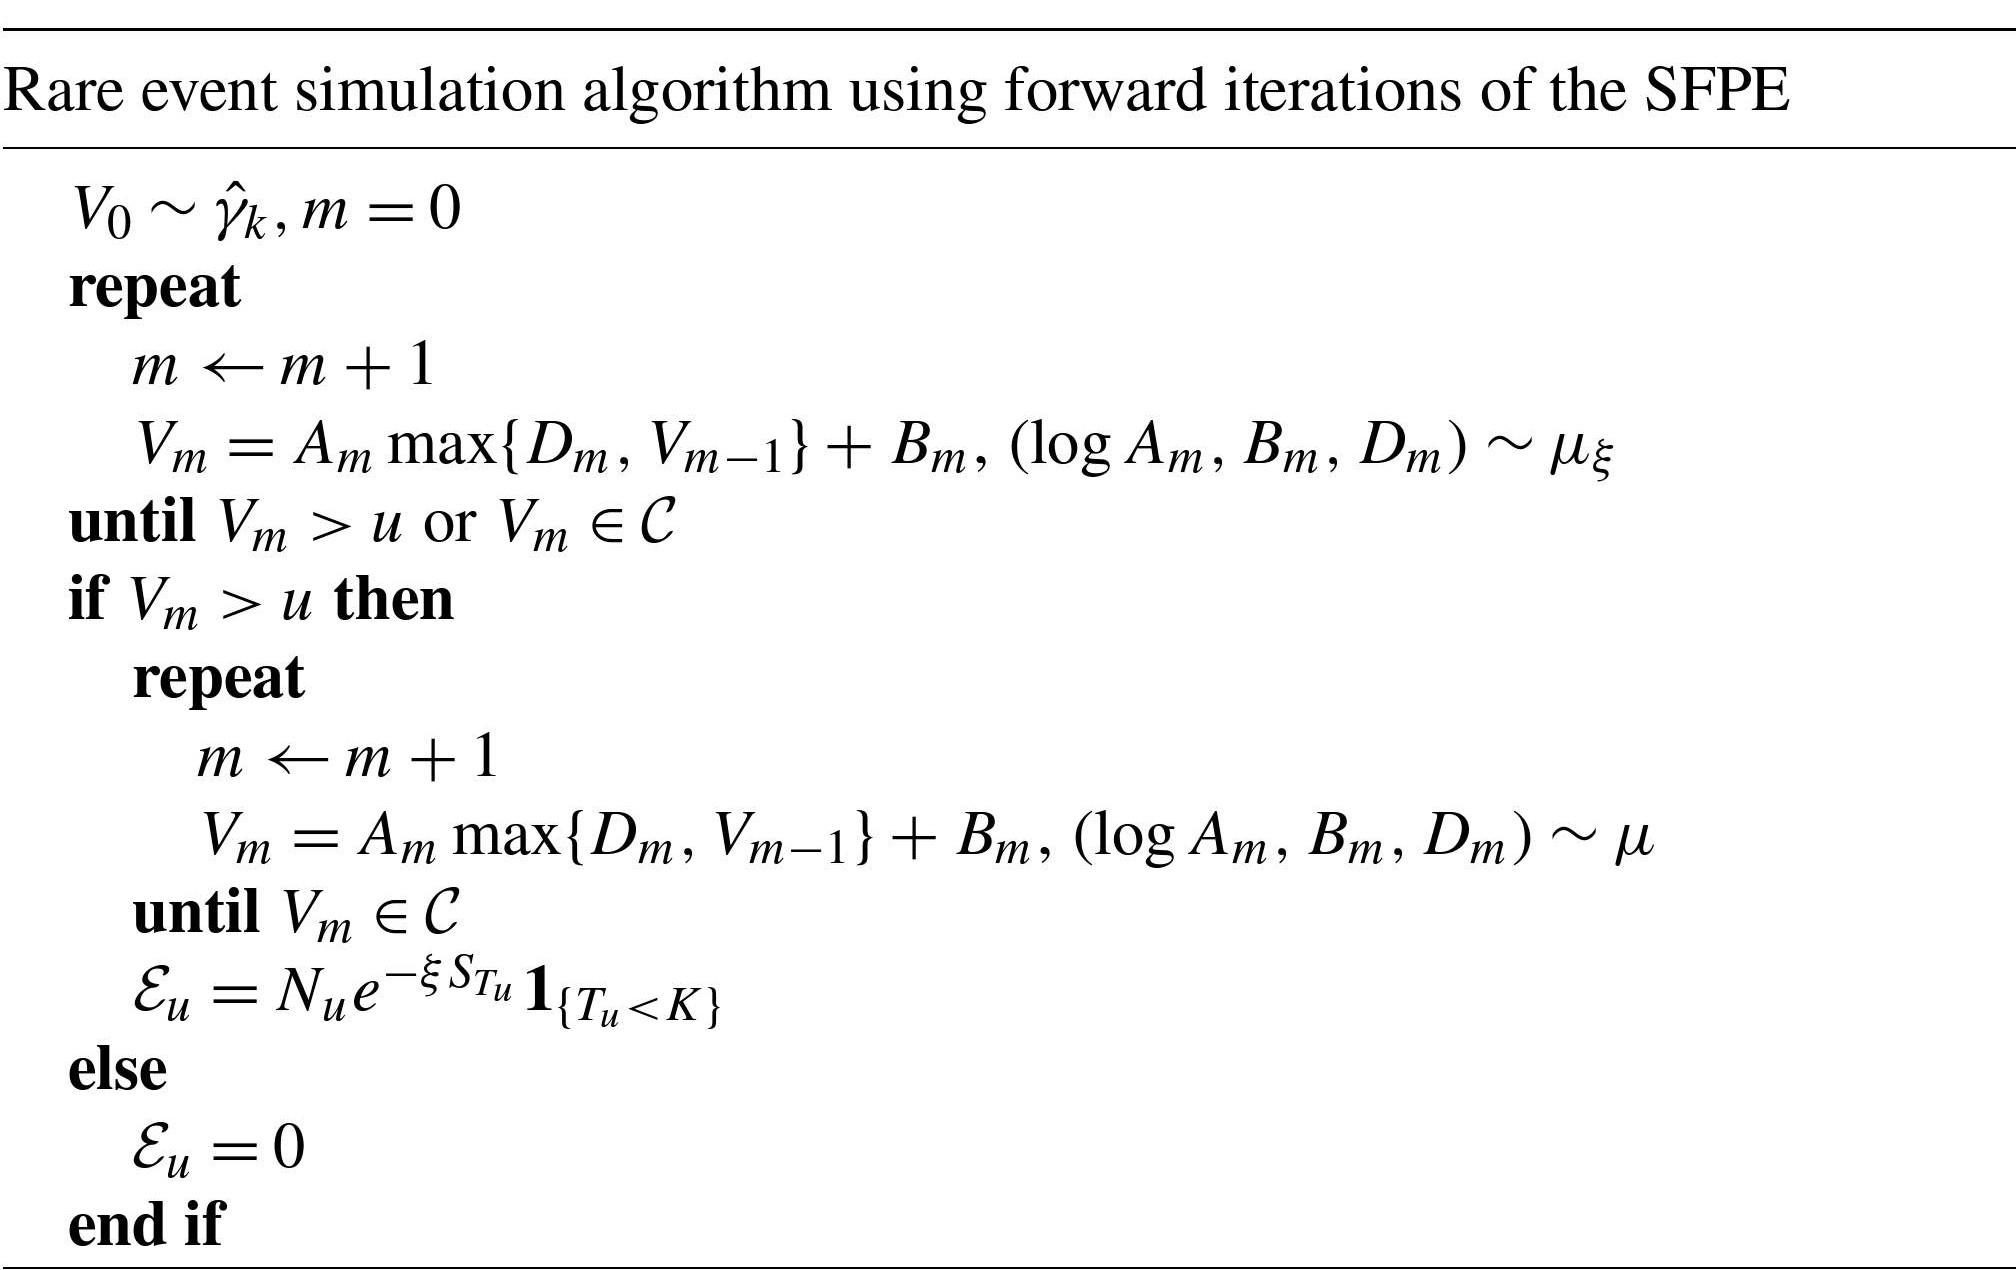
\includegraphics[scale=0.14]{IMG_1091.jpg}
  \end{figure}
\end{frame}

\begin{frame}
  Intuitively
  \[
  \P(V > u) = {
    \E N_u
    \over
    \E K
  }
  \]
  where $K$ is a typical return time to the set $\mathcal C$ and
  \[
  N_u = \sum_{i=1}^{K - 1} \1{V > u}
  \]
  It is straight forward to show $\E K = 1/\pi(\mathcal C)$. We need to
  have an efficient estimator for $\E N_u$.
\end{frame}


%% \section{Setup of the Problem}

% \begin{frame}
%   The recurrent property of a geometriclly ergodic MC means imples the
%   process the MC has a regeneration structure \cite{Nummelin1978}:
%   There exist random times $1 \leq T_1 < T_2 < \cdots$ such that
%   \begin{enumerate}
%   \item $T_0, T_{i+1} - T_{i}$, $i = 1, 2, \cdots$ are finite with
%     probability 1 and are independent, identically distributed random
%     variables.
%   \item The blocks $(V_{T_i}, \dots, V_{T_{i+1} - 1})$ are independent;
%   \item $\P(V_{T_i} \in A | V_{T_{i}-1}, \dots, V_0 = \nu(A)$
%   \end{enumerate}
% \end{frame}

\section{Sketch of the Proof of Efficiency}
\begin{frame}
  To show that the estimator is efficient, we need to show
  \[
  \lim_{u \to \infty} {
    \var_{\mathcal D}(\mathcal E_u)
    \over
    (\E_{\mathcal D} \mathcal E_u)^2
  } < \infty
  \]
  Because
  \[
  \lim_{u \to \infty} u^\xi \P(V > u) = C
  \]
  It suffices to show
  \[
  \lim_{u \to \infty}
    \E_{\mathcal D}(\mathcal E_u^2 u^{2\xi}) < \infty
  \]
\end{frame}

\begin{frame}
  \frametitle{Drift towards set $\mathcal C$}
  We need to prove a lemma first:
  \begin{exampleblock}{Drift Condition}
    A drift condition: Given $\lambda_\beta(\alpha) = \E_\beta
    A^\alpha < \infty$,
    \[
    \E_\beta (|V_n|^\alpha \I{\mathcal C^\complement}(V_{n-1}) |
    V_{n-1}) < \rho |V_{n-1}|^\alpha\I{\mathcal C^\complement}(V_{n-1})
    \]
    for some $\rho > \lambda_\beta(\alpha)$ and some constant $M > 0$,
    $\mathcal C = (-M, M)$.
  \end{exampleblock}
\end{frame}

\begin{frame}
  \frametitle{Proof of the drift condition}
  We'll use the lemma for $\lambda_\beta(\alpha) < 1$. for
  simplicity, assume $\alpha < 1$. By subadditivity
  \[
  |V_n|^\alpha \leq A_n^\alpha |V_{n-1}|^\alpha + |\tilde B_n|^\alpha
  \]
  Hence
  \begin{eqnarray*}
    && \E_\beta (|V_n|^\alpha \I{\mathcal C^\complement}(V_{n-1})
    | V_{n-1}) \\
    &\leq& \E_\beta A_n^\alpha |V_{n-1}|^\alpha +
    \E_\beta |\tilde B_n|^\alpha \\
    &=& |V_{n-1}|^\alpha \left[
      \lambda_\beta(\alpha) + {
        \E_\beta |\tilde B_n|^\alpha
        \over
        |V_{n-1}|^\alpha
      }
    \right]
  \end{eqnarray*}
  Clearly, for any $\epsilon > 0$, we may choose $M$ sufficiently
  large such that $V_{n-1} \in \mathcal C^\complement$ imples
  $|V_n|^\alpha < |V_{n-1}|^\alpha (\lambda_\beta (\alpha) + \epsilon)$.
\end{frame}

\begin{frame}
  \frametitle{An upper bound on $\P(K > n)$}
  Iterating the drift condition gives
  \begin{eqnarray*}
    \E_\beta |V_n|^\alpha
    \1{V_{n-1}, \dots, V_1 \in \mathcal C^\complement}
    &\leq& |V_1|^\alpha [a \lambda_\beta(\alpha)]^{n-1}
    \1{V_{n-1}, \dots, V_1 \in \mathcal C^\complement}
  \end{eqnarray*}
  for some $a > 1$. Even smaller than the LHS is $\E_\beta |V_n|^\alpha
  \1{V_n, \dots, V_1 \in \mathcal C^\complement}$. $V_n \in \mathcal
  C^\complement$ means $K > n$ and $|V_n| > M$. Thus
  \[
  \P_\beta(K > n) \leq {
    |V_1|^\alpha
    \over
    M^\alpha
  } [a \lambda_\beta(\alpha)]^{n-1}
  \]
  for any $a > 1$ and $M$ sufficiently large. Note $|V_1|^\alpha <
  \infty$ a.s. under assumption $\E A^\alpha < \infty$.
\end{frame}

\begin{frame}
  First consider the case $\lambda(-\alpha) < \infty$ for some $\alpha
  > \xi$. Using
  \begin{eqnarray*}
    V_{T_u} &>& u \\
    {V_{T_u}
      \over
      A_{T_u} \cdots A_0
    } &\leq& \sum_{n=0}^{T_u} {
      \tilde B_n
      \over
      A_n \cdots A_0
    }
  \end{eqnarray*}
  where $A_{0} := 1$, $A_i$ for $i =1, 2, \dots$ are iid and $\tilde B_n :=
  A_n |D_n| + |B_n|$. We get
  \[
  \E_{\mathcal D}(\mathcal E_u^2 u^{2\xi}) \leq
  \E_{\mathcal D} \left[
    N_u^2
    \left(
    \sum_{n=0}^{\infty} {
      \tilde B_n
      \over
      |A_n \cdots A_0|
    }
    \1{n \leq T_u < K}
    \right)^{2\xi}
    \right]
  \]
\end{frame}

\begin{frame}
  If $\xi \geq 1/2$, applying Minkowski's inequality, changing to
  the original measure and then using H\"older's inequality gives
  \begin{eqnarray*}
    (u^{2\xi} \E_{\mathcal D} \mathcal{E}^{2\xi}_u)^{1/2\xi} &\leq&
    \sum_{n=0}^\infty
    (\E N_u^{2r} \1{n-1 < T_u \wedge K})^{1/2r\xi} \times \\
    && [\E (A_n^{-1} \tilde B_n^2)^{s\xi}]^{1/2s\xi} \times \\
    && \E[
    (A_{n-1} \cdots A_0)^{-s\xi}
    \1{n-1 < T_u \wedge K}
    ]^{1/2s\xi}
  \end{eqnarray*}
  For the last term on RHS, change to the $-s\xi$ shifted measure to
  obtain
  \[
  \E[
    (A_{n-1} \cdots A_0)^{-s\xi}
    \1{n-1 < T_u \wedge K}
    ]^{1/2s\xi} = \lambda(-s\xi)^{n-1} \P_{-s\xi}(n-1 < T_u \wedge K)
  \]
\end{frame}

\begin{frame}
  Using the {\it drift condition} in the $-s\xi$-shifted measure leads to
  \begin{eqnarray*}
    \P_{-s\xi}(n-1 < T_u \wedge K) &\leq& C
    \lambda_{-s\xi}(\alpha)^{n-1} \\
    &=& C \left[
      {
      \lambda(-s\xi + \alpha)
      \over
      \lambda(-s\xi)
    }
    \right]^{n-1}. \\
    \lambda(-s\xi)^{n-1} \P_{-s\xi}(n-1 < T_u \wedge K) &\leq& C
    \lambda(-s\xi + \alpha)^{n-1}
  \end{eqnarray*}
  for some $0 < \alpha < \xi$. By assumption $\lambda(-s\xi) < \infty$
  and hence $\alpha$ can be chosen such that $\lambda(-s\xi + \alpha)
  < 1$.
\end{frame}

\begin{frame}
  As for $\E N_u^{2r}$, first notice
  \[
  N_u = \sum_{i=0}^{K-1} \1{V_i > u} \leq K
  \]
  Hence
  \begin{eqnarray*}
    \E N_u^{2r}\1{n-1 \leq T_u < K} &\leq& \sum_{i=n}^\infty i^{2r}
    \P(K > i-1) \\
    &\leq& c \sum_{i=n}^\infty i^{2r} \lambda(\alpha)^i < \infty
  \end{eqnarray*}
  for some constant $c$ and $\alpha$ chosen such that $\lambda(\alpha)
  < 1$.
\end{frame}

\begin{frame}
  The case $\xi < 1/2$ is proven analogously by exploiting
  subadditivity of the function $(\cdot)^{2\xi}$ in place of
  Minkowski's inequality. The somewhat more complicated case
  $\lambda(-\xi) = \infty$ is proven with an extra assumption
  \[
  \E (A^{-1} \tilde B)^\alpha < \infty
  \]
  for all $\alpha > 0$. First notice when $n \leq T_u < K$
  \begin{eqnarray*}
    |V_n| &\leq& A_n |V_{n-1}| \left(
      1 + {
        \tilde B_n
        \over
        A_n |V_{n-1}|
      }
    \right)
  \end{eqnarray*}
  and $M \leq V_n < u$. Hence
  \[
  A_n^{-s\xi} \leq \left(
    {
      u \over M
    }
    \right)^{s\xi} 
    \left(
    1 + {
      \tilde B_n
      \over
      A_n M
    }
  \right)^{s\xi}
  \]
\end{frame}

\begin{frame}
  Since by assumption $\E (A_n^{-1} \tilde B_n)^{s\xi} < \infty$, we
  have
  \[
  \E (A_{n} \cdots A_0)^{-s\xi} < \infty
  \]
  for fixed $n \leq T_u$. Then it suffices to show
  \[
  \sum_{n=0}^\infty {
    \E (A_n \cdots A_0)^{-s\xi} \1{n \leq T_u < K}
  } < \infty
  \]
  The proof of finiteness of the other terms are identical to that in
  the other case.
\end{frame}

\begin{frame}
  Let $\zeta = s \xi$. Define a sequence $L_k \to 0$ as $k \to \infty$
  and
  \[
  \E {
    1 \over
    (A_k \cdots A_0)^\zeta
  }  \1{F_k} < {1 \over k^2}
  \]
  where $F_k$ denotes the event $A_1, A_2, \dots, A_{k} \geq
  L_k$. Clearly
  \[
  \sum_{k=0}^\infty  \E {
    1 \over
    (A_k \cdots A_0)^\zeta
  }  \1{F_k} <  \sum_{k=1}^\infty {1 \over k^2} < \infty
  \]
  It remains to show
  \[
  \sum_{k=0}^\infty  \E {
    1 \over
    (A_k \cdots A_0)^\zeta
  }  \1{F_k^\complement} \1{k \leq T_u < K} < \infty
  \]
\end{frame}

\begin{frame}
  Let
  \begin{eqnarray*}
    \bar A_{n,k} &=& A_{n} \1{A_n \geq L_k} + L_k \1{A_n < L_k} \\
    \lambda_k(\alpha) &=& \E \bar A_{1,k}^\alpha
  \end{eqnarray*}
  By changing to the $-\zeta$ shifted measure, we obtain
  \[
  \E {
    1\over
    (A_k \cdots A_0)^\zeta
  } \1{F_k^\complement} \1{k \leq T_u < K}
  \leq \E_{-\zeta}(\1{F_k^\complement} \1{k \leq T_u < K})
  \lambda_k(-\zeta)^{k-1} 
  \]
\end{frame}

\begin{frame}
  Observe that $\bar A_{n,k} \to A_n$ and $\lambda_k(\alpha) \to
  \lambda(\alpha)$ as $k \to \infty$. By Minkowski's inequality
  followed by H\"older's inequality, we obtain
  \begin{eqnarray*}
    \E_{-s\xi} \left( |V_{1,k}|^\beta | V_{0,k} = w\right) &\leq& {
    t [\E \bar A_{1,k}^{p(\beta - \zeta)}]^{1/p}
    \over
    \lambda_k(-\zeta)
  } w^\beta \times \\
  && \left\{
    t^{-q} \E \left[
      1 + {
        \tilde B_1
        \over
        w \bar A_{1,k}
      }
    \right]^{q\beta}
  \right\}^{1/q}
  \end{eqnarray*}
  for some $t > 1$. Notice that $p > 1$ may be chosen so close to 1
  and $\beta$ chosen appropriately so that
  \[
  \E \bar A_{1,k}^{p(\beta - \zeta)} < \rho < 1 \text{ for all } k > k_0
  \]
\end{frame}

\begin{frame}
  Such a choice is possible because $\lambda_{1,k}(p(\beta - \zeta))
  \to \lambda(p(\beta - \zeta))$ and
  \[
  \inf_{\alpha > 1} \lambda(\alpha) < 1
  \]
  Choose $M$ sufficiently large so that $\forall w > M$,
  \[
    t^{-q} \E \left[
      1 + {
        \tilde B_1
        \over
        w \bar A_{1,k}
      }
    \right]^{q\beta} < 1
  \]
  So we have obtained an inequality similar to the drift condition in
  the $\lambda(-\xi) < \infty$ case.  Iterating this inequality gives
  \[
  \E_{-\zeta}(\1{F_k^\complement} \1{k \leq T_u < K}) \leq b \left[
  {
    a \lambda (p(\beta - \zeta))
    \over
    \lambda(-\zeta)
  }
\right]^{k-1}
  \]
  for some $b < \infty$ a.s. and any $a > 1$. Hence
  \[
  \sum_{k=0}^\infty \E {
    1 \over
    (A_k \cdots A_0)^\zeta
  }  \1{F_k}  \1{n \leq T_u < K}
  <
  b \sum_{k=0}^\infty \left[
  {
    a \lambda (p(\beta - \zeta))
  }
\right]^{k-1} < \infty
  \]

\end{frame}

\section{Sketch of the Proof of Consistency}
% \begin{frame}
%   \frametitle{Does the algorithm give correct estimates?}
%   A recurrent MC is also positive, i.e. it admits an invariant
%   measure $\pi$ \cite{Meyn:2009:MCS:1550713}:
%   \[
%   \pi(A) = \int_E \pi(dx) P(x, A)
%   \]
%   for all $A \in \mathcal B(E)$.
%   By geometric ergodicity, $V_n$ converges to a random variable $V$
%   distributed according to $\pi$. We want to have an efficient estimator of the
%   probability $\P(V > u)$ as $u \to \infty$. It is understood
%   \[
%    \lim_{u \to \infty} u^\xi \P(V > u) = C
%   \]
%   for some constant $C > 0$.
% \end{frame}

% \begin{frame}
%   Collamore and Vidyashankar \cite{collamore2014} showed, when
%   $V_0$ is in the set $\mathcal C$ and is distributed according to
%   $\gamma$ defined as
%   \[
%   \gamma(E) = \pi(E)/\pi(\mathcal C)\text{ for all } E \in \mathcal B(\mathcal C)
%   \]
%   $\mathcal E_u = \pi(\mathcal C) N_u |A_{T_u} \cdots A_{1}
%   V_0|^{-\xi}\1{T_u < \tau}$ is an unbiased and efficient estimator
%   w.r.t the dual measure $\mathcal D$:
%   \[
%   \E_{\mathcal D} E_u = \P(V > u)
%   \]
%   and by ``efficient'' we mean
%   \[
%   \lim_{u \to \infty} {
%     \var_{\mathcal D}(\mathcal E_u)
%     \over
%     (\E_{\mathcal D} \mathcal E_u)^2
%   } < \infty
%   \]
%   as defined by Asmusen \cite{opac-b1123521}.
%   \begin{eqnarray*}
%     K &:=& \inf\{n \geq 1: V_n \in \mathcal C\} \\
%     T_u &:=& \min\{n \geq 1: V_n > u\} \\
%     N_u &:=& \sum_{n=0}^{K-1} \1{V_n > u}
%   \end{eqnarray*}
% \end{frame}

\begin{frame}
  \frametitle{Does the algorithm give correct estimates?}
  \begin{exampleblock}{theorem}
  \[
  \lim_{k \to \infty} \lim_{n \to \infty} \hat{\pi}_k \hat{\mathcal
    E}_{u,n} = \P(V > u)
  \]
  \end{exampleblock}
  What follows is a sketch of the proof by Collamore, Guoqing and
  Vidyashankar \cite{collamore2014}. By the law of large numbers for
  Markov chains
  \[
  \P(V > u) = \lim_{n \to \infty} {1 \over n} \left\{
  \sum_{i=0}^{K_{R_n} - 1} \1{V_i > u}
  +
  \sum_{i=K_{R_n}}^{n} \1{V_i > u}
  \right\}
  \]
  where $K_0 = 0$ and $K_n$ is the time of the $n$-th visit to
  $\mathcal C$. $R_n = \sum_{i=1}^n \1{V_i \in C}$ is the number of
  visits to $\mathcal C$ before time $n$.
\end{frame}

\begin{frame}
  By the Markov renewal theorem and the geometric ergodicity of $V_n$,
  \[
  \lim_{n \to \infty} e^{\epsilon(J(n) - I(n))} = {
    \E \tau e^{\epsilon \tau}
    \over
    \E \tau
  }  < \infty
  \]
  where $\tau$ is a typical regeneration time, $I(n)$ is the last
  regeneration time before time $n$ and $J(n)$ the first regeneration
  time after $n$. Then by a Borel-Cantelli argument
  \[
  {1 \over n}\sum_{i=K_{R_n}}^n \1{V_i > u} \to 0
  \]
\end{frame}

\bibliographystyle{unsrt}
\bibliography{../../thesis/econophysics}
\end{document} 

